% 레거시 원본: PDF 실습 1, p.3--52. 본문과 사진을 보존한다.
% 생성 후 직접 편집 가능. 이미지와 출처 대응: assets/legacy-01/README.md
\section{레거시 01: 논리 게이트}

\begin{frame}[label=legacy-01-vivado]{레거시 01 · 논리 게이트}
\small

{\large\bfseries [실습 1] AND, OR, XOR 게이트 구현}\par\vspace{0.35cm}
\begin{itemize}
\item 입력 \texttt{a, b}에 대한 출력 \texttt{x, y, z}를 확인한다.
\item 원본의 프로젝트 이름: \texttt{logic\_gate}.
\item 대상 부품: Spartan-7 \texttt{xc7s75fgga484-1}.
\end{itemize}
\vspace{0.35cm}
{\color{UOSBlue}\bfseries 실습 순서}\par\vspace{0.12cm}
VS Code 사전 시뮬레이션·실험 전 레포트\par
Vivado 실습·FPGA 기록·동작 확인\par
사진·영상·GitHub·실험 후 레포트
\vspace{0.35cm}\par
{\scriptsize 작성일 \materialdate\quad\presenter\par
원자료: 박동욱 교수, 서울시립대학교, 「논리 게이트 구현」.\par
다음 원문 페이지는 2022년 보관 PDF의 사진과 설명을 재구성했다.}

\legacySource{3}
\end{frame}

\begin{frame}[label=legacy-01-vivado-contents]{레거시 01 · Vivado 목차}
\small

\begin{tabular}{@{}ll@{}}
\navlink{legacy-01-p04}{설계 기획} & 블록도·진리표\\[0.15cm]
\navlink{legacy-01-p05}{(1) 프로젝트 선언} & 부품·경로·프로젝트 설정\\[0.15cm]
\navlink{legacy-01-p12}{(2) 로직 설계} & 원본 코드·소스 등록\\[0.15cm]
\navlink{legacy-01-p19}{(3) Assignment} & 입출력 핀·전기 규격\\[0.15cm]
\navlink{legacy-01-p28}{(4) Compile} & 합성·배치배선\\[0.15cm]
\navlink{legacy-01-p34}{(5) Simulation} & 테스트벤치·파형\\[0.15cm]
\navlink{legacy-01-p44}{(6) Programming} & 비트스트림·실제 장치 기록\\[0.15cm]
\navlink{legacy-01-p52}{(7) 동작 확인} & 스위치 입력·LED 출력
\end{tabular}
\vspace{0.35cm}\par
{\scriptsize 원본 순서를 보존했다. 수업에서는 합성·구현에 앞서 VS Code와\par
Vivado에서 시뮬레이션한다. \navlink{legacy-01-notes}{원문 보충 설명} ·
\navlink{lab1-reports}{실험 전·후 레포트} ·
\href{run:README.md}{자료 안내}}

\end{frame}

\begin{frame}[label=legacy-01-p04]{설계 기획}
\small
{\color{UOSBlue}\bfseries 블록도 및 진리표}\par\vspace{0.5cm}
\centering\includegraphics[width=\textwidth]{assets/legacy-01/p004-diagram-truth-table.png}
\legacySource{4}
\end{frame}

\begin{frame}[label=legacy-01-p05]{로직 설계 및 합성}
\small
{\color{UOSBlue}\bfseries (1) 프로젝트 선언}\par\vspace{0.12cm}
\begin{itemize}
\setlength{\itemsep}{0.08cm}
\item {Vivado 실행}
\item {File \textgreater{} Project \textgreater{} New}
\end{itemize}
\par\vspace{0.12cm}
{\centering
\includegraphics[width=\textwidth,height=4.15cm,keepaspectratio]{assets/legacy-01/p005-01.png}
\par}
\legacySource{5}
\end{frame}

\begin{frame}[label=legacy-01-p06]{로직 설계 및 합성}
\small
{\color{UOSBlue}\bfseries (1) 프로젝트 선언}\par\vspace{0.12cm}
\begin{itemize}
\setlength{\itemsep}{0.08cm}
\item {Next}
\end{itemize}
\par\vspace{0.12cm}
{\centering
\includegraphics[width=\textwidth,height=4.6cm,keepaspectratio]{assets/legacy-01/p006-01.png}
\par}
\legacySource{6}
\end{frame}

\begin{frame}[label=legacy-01-p07]{로직 설계 및 합성}
\small
{\color{UOSBlue}\bfseries (1) 프로젝트 선언}\par\vspace{0.12cm}
\begin{itemize}
\setlength{\itemsep}{0.08cm}
\item {Project Name과 Project Location 설정}
\item {Project Name : logic\_gate}
\item {Project location : d:/work}
\item {Create project subdirectory : 체크}
\item {d:/work 폴더에 logic\_gate 폴더를 생성}
\end{itemize}
\legacySource{7}
\end{frame}

\begin{frame}{로직 설계 및 합성}
\small
{\color{UOSBlue}\bfseries (1) 프로젝트 선언}\par\vspace{0.12cm}
{\scriptsize 원문 설명에 대응하는 실제 화면}\par
\par\vspace{0.12cm}
{\centering
\includegraphics[width=\textwidth,height=4.6cm,keepaspectratio]{assets/legacy-01/p007-01.png}
\par}
\legacySource{7}
\end{frame}

\begin{frame}[label=legacy-01-p08]{로직 설계 및 합성}
\small
{\color{UOSBlue}\bfseries (1) 프로젝트 선언}\par\vspace{0.12cm}
\begin{itemize}
\setlength{\itemsep}{0.08cm}
\item {Project Type 설정}
\item {RTL Project}
\end{itemize}
\par\vspace{0.12cm}
{\centering
\includegraphics[width=\textwidth,height=4.15cm,keepaspectratio]{assets/legacy-01/p008-01.png}
\par}
\legacySource{8}
\end{frame}

\begin{frame}[label=legacy-01-p09]{로직 설계 및 합성}
\small
{\color{UOSBlue}\bfseries (1) 프로젝트 선언}\par\vspace{0.12cm}
\begin{itemize}
\setlength{\itemsep}{0.08cm}
\item {Add source와 Add Constraints 설정}
\item {설계된 로직 파일과 설정된 핀 정보 파일이 없기 때문에 Next 버튼 누름.}
\end{itemize}
\par\vspace{0.12cm}
{\centering
\includegraphics[width=\textwidth,height=4.15cm,keepaspectratio]{assets/legacy-01/p009-01.png}
\par}
\legacySource{9}
\end{frame}

\begin{frame}{로직 설계 및 합성}
\small
{\color{UOSBlue}\bfseries (1) 프로젝트 선언}\par\vspace{0.12cm}
\begin{itemize}
\setlength{\itemsep}{0.08cm}
\item {Add source와 Add Constraints 설정}
\item {설계된 로직 파일과 설정된 핀 정보 파일이 없기 때문에 Next 버튼 누름.}
\end{itemize}
\par\vspace{0.12cm}
{\centering
\includegraphics[width=\textwidth,height=4.15cm,keepaspectratio]{assets/legacy-01/p009-02.png}
\par}
\legacySource{9}
\end{frame}

\begin{frame}[label=legacy-01-p10]{로직 설계 및 합성}
\small
{\color{UOSBlue}\bfseries (1) 프로젝트 선언}\par\vspace{0.12cm}
\begin{itemize}
\setlength{\itemsep}{0.08cm}
\item {Device 설정}
\item {Family : Spartan-7}
\item {Part : xc7s75fgga484-1}
\end{itemize}
\legacySource{10}
\end{frame}

\begin{frame}{로직 설계 및 합성}
\small
{\color{UOSBlue}\bfseries (1) 프로젝트 선언}\par\vspace{0.12cm}
{\scriptsize 원문 설명에 대응하는 실제 화면}\par
\par\vspace{0.12cm}
{\centering
\includegraphics[width=\textwidth,height=4.6cm,keepaspectratio]{assets/legacy-01/p010-01.png}
\par}
\legacySource{10}
\end{frame}

\begin{frame}[label=legacy-01-p11]{로직 설계 및 합성}
\small
{\color{UOSBlue}\bfseries (1) 프로젝트 선언}\par\vspace{0.12cm}
\begin{itemize}
\setlength{\itemsep}{0.08cm}
\item {설정된 Summary 확인.}
\item {Finish를 눌러 프로젝트 선언 완료}
\end{itemize}
\par\vspace{0.12cm}
{\centering
\includegraphics[width=\textwidth,height=4.15cm,keepaspectratio]{assets/legacy-01/p011-01.png}
\par}
\legacySource{11}
\end{frame}

\begin{frame}[label=legacy-01-p12]{로직 설계 및 합성}
\small
{\color{UOSBlue}\bfseries (2) 로직 설계}\par\vspace{0.12cm}
\begin{itemize}
\setlength{\itemsep}{0.08cm}
\item {VIVADO 프로그램}
\item {Text Editor \textgreater{} New File.. 선택}
\end{itemize}
\par\vspace{0.12cm}
{\centering
\includegraphics[width=\textwidth,height=4.15cm,keepaspectratio]{assets/legacy-01/p012-01.png}
\par}
\legacySource{12}
\end{frame}

\begin{frame}[label=legacy-01-p13]{로직 설계 및 합성}
\small
{\color{UOSBlue}\bfseries (2) 로직 설계}\par\vspace{0.12cm}
\begin{itemize}
\setlength{\itemsep}{0.08cm}
\item {logic\_gate.v 파일로 저장}
\end{itemize}
\par\vspace{0.12cm}
{\centering
\includegraphics[width=\textwidth,height=4.6cm,keepaspectratio]{assets/legacy-01/p013-01.png}
\par}
\legacySource{13}
\end{frame}

\begin{frame}[label=legacy-01-p14]{로직 설계 및 합성}
\small
{\color{UOSBlue}\bfseries (2) 로직 설계}\par\vspace{0.12cm}
\begin{itemize}
\setlength{\itemsep}{0.08cm}
\item {로직 설계}
\end{itemize}
\par\vspace{0.12cm}
{\centering
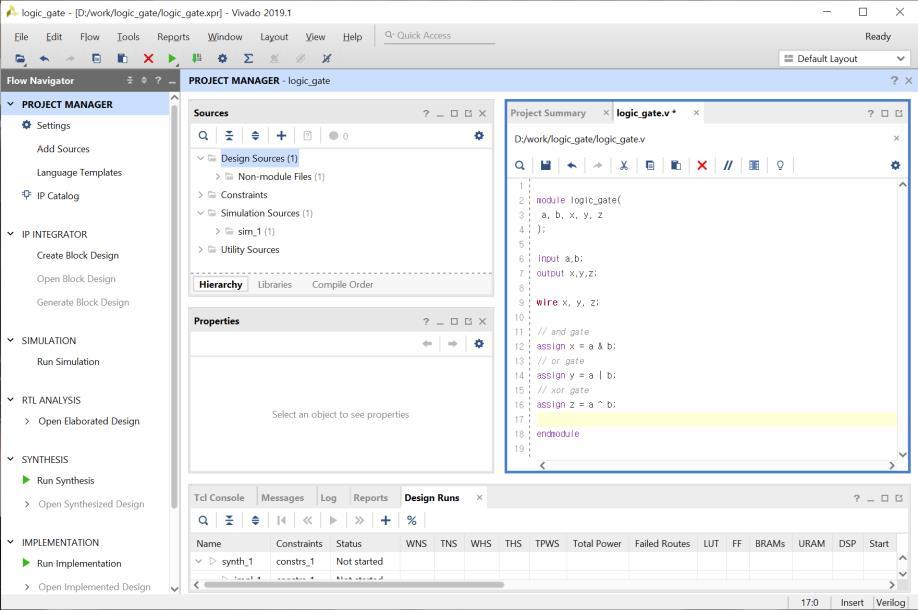
\includegraphics[width=\textwidth,height=4.6cm,keepaspectratio]{assets/legacy-01/p014-01.jpg}
\par}
\legacySource{14}
\end{frame}

\begin{frame}{로직 설계 및 합성}
\small
{\color{UOSBlue}\bfseries (2) 로직 설계}\par\vspace{0.12cm}
\begin{itemize}
\setlength{\itemsep}{0.08cm}
\item {로직 설계}
\end{itemize}
\par\vspace{0.12cm}
{\centering
\includegraphics[width=\textwidth,height=4.6cm,keepaspectratio]{assets/legacy-01/p014-02.png}
\par}
\legacySource{14}
\end{frame}

\begin{frame}[label=legacy-01-p15]{로직 설계 및 합성}
\small
{\color{UOSBlue}\bfseries (2) 로직 설계}\par\vspace{0.12cm}
\begin{itemize}
\setlength{\itemsep}{0.08cm}
\item {PROJECT MANAGER \textgreater{} Add Sources 선택}
\end{itemize}
\par\vspace{0.12cm}
{\centering
\includegraphics[width=\textwidth,height=4.6cm,keepaspectratio]{assets/legacy-01/p015-01.png}
\par}
\legacySource{15}
\end{frame}

\begin{frame}[label=legacy-01-p16]{로직 설계 및 합성}
\small
{\color{UOSBlue}\bfseries (2) 로직 설계}\par\vspace{0.12cm}
\begin{itemize}
\setlength{\itemsep}{0.08cm}
\item {Add Sources 창에서 Add or Create design sources 선택}
\end{itemize}
\par\vspace{0.12cm}
{\centering
\includegraphics[width=\textwidth,height=4.6cm,keepaspectratio]{assets/legacy-01/p016-01.png}
\par}
\legacySource{16}
\end{frame}

\begin{frame}[label=legacy-01-p17]{로직 설계 및 합성}
\small
{\color{UOSBlue}\bfseries (2) 로직 설계}\par\vspace{0.12cm}
\begin{itemize}
\setlength{\itemsep}{0.08cm}
\item {Add Files 버튼을 눌러, 앞의 logic\_gate.v 파일 추가}
\end{itemize}
\par\vspace{0.12cm}
{\centering
\includegraphics[width=\textwidth,height=4.6cm,keepaspectratio]{assets/legacy-01/p017-01.png}
\par}
\legacySource{17}
\end{frame}

\begin{frame}{로직 설계 및 합성}
\small
{\color{UOSBlue}\bfseries (2) 로직 설계}\par\vspace{0.12cm}
\begin{itemize}
\setlength{\itemsep}{0.08cm}
\item {Add Files 버튼을 눌러, 앞의 logic\_gate.v 파일 추가}
\end{itemize}
\par\vspace{0.12cm}
{\centering
\includegraphics[width=\textwidth,height=4.6cm,keepaspectratio]{assets/legacy-01/p017-02.png}
\par}
\legacySource{17}
\end{frame}

\begin{frame}[label=legacy-01-p18]{로직 설계 및 합성}
\small
{\color{UOSBlue}\bfseries (2) 로직 설계}\par\vspace{0.12cm}
\begin{itemize}
\setlength{\itemsep}{0.08cm}
\item {Sources 창에서 파일 추가된 것을 확인}
\end{itemize}
\par\vspace{0.12cm}
{\centering
\includegraphics[width=\textwidth,height=4.6cm,keepaspectratio]{assets/legacy-01/p018-01.png}
\par}
\legacySource{18}
\end{frame}

\begin{frame}[label=legacy-01-p19]{로직 설계 및 합성}
\small
{\color{UOSBlue}\bfseries (3) Assignment}\par\vspace{0.12cm}
\begin{itemize}
\setlength{\itemsep}{0.08cm}
\item {프로젝트의 타겟이 되는 FPGA 디바이스와 설계된 로직에서 사용하는 입출력 단자를 하드웨어와 연결하기 위하여 핀을 설정하는 것}
\end{itemize}
\legacySource{19}
\end{frame}

\begin{frame}[label=legacy-01-p20]{로직 설계 및 합성}
\small
{\color{UOSBlue}\bfseries (3) Assignment}\par\vspace{0.12cm}
\begin{itemize}
\setlength{\itemsep}{0.08cm}
\item {PROJECT MANAGER의 RTL ANALYSIS 탭의 Open Elaborated Design 부분을 마우스로 클릭}
\end{itemize}
\par\vspace{0.12cm}
{\centering
\includegraphics[width=\textwidth,height=4.6cm,keepaspectratio]{assets/legacy-01/p020-01.png}
\par}
\legacySource{20}
\end{frame}

\begin{frame}[label=legacy-01-p21]{로직 설계 및 합성}
\small
{\color{UOSBlue}\bfseries (3) Assignment}\par\vspace{0.12cm}
\begin{itemize}
\setlength{\itemsep}{0.08cm}
\item {메시지 창이 나타난다.}
\item {OK 버튼을 누르면 Elaboration 과정이 진행됨.}
\item {문법에 오류부분도 같이 체크하여 오류가 있다면 에러 메시지가 출력됨.}
\end{itemize}
\legacySource{21}
\end{frame}

\begin{frame}{로직 설계 및 합성}
\small
{\color{UOSBlue}\bfseries (3) Assignment}\par\vspace{0.12cm}
{\scriptsize 원문 설명에 대응하는 실제 화면}\par
\par\vspace{0.12cm}
{\centering
\includegraphics[width=\textwidth,height=4.6cm,keepaspectratio]{assets/legacy-01/p021-01.png}
\par}
\legacySource{21}
\end{frame}

\begin{frame}[label=legacy-01-p22]{로직 설계 및 합성}
\small
{\color{UOSBlue}\bfseries (3) Assignment}\par\vspace{0.12cm}
\begin{itemize}
\setlength{\itemsep}{0.08cm}
\item {설계된 Verilog HDL 구문이 Schematic으로 표현되는 것을 확인}
\end{itemize}
\par\vspace{0.12cm}
{\centering
\includegraphics[width=\textwidth,height=4.6cm,keepaspectratio]{assets/legacy-01/p022-01.png}
\par}
\legacySource{22}
\end{frame}

\begin{frame}[label=legacy-01-p23]{로직 설계 및 합성}
\small
{\color{UOSBlue}\bfseries (3) Assignment}\par\vspace{0.12cm}
\begin{itemize}
\setlength{\itemsep}{0.08cm}
\item {Schematic 화면 오른 쪽 윗 부분의 5 I/O Ports 선택}
\end{itemize}
\par\vspace{0.12cm}
{\centering
\includegraphics[width=\textwidth,height=4.6cm,keepaspectratio]{assets/legacy-01/p023-01.png}
\par}
\legacySource{23}
\end{frame}

\begin{frame}[label=legacy-01-p24]{로직 설계 및 합성}
\small
{\color{UOSBlue}\bfseries (3) Assignment}\par\vspace{0.15cm}\begin{itemize}
\setlength{\itemsep}{0.08cm}
\item {I/O Std를 “LVCMOSS33” 으로 변경}
\item {입/출력 포트의 Voltage Level을 3.3V로 설정하는 것.}
\end{itemize}
\vspace{0.5cm}\centering
\renewcommand{\arraystretch}{1.45}
\begin{tabular}{ccc|ccc}
포트 이름 & 핀 번호 & & 포트 이름 & 핀 번호 &\\\hline
\texttt{a} & K4 & SW\_1 & \texttt{x} & L4 & LED1\\
\texttt{b} & N8 & SW\_2 & \texttt{y} & M4 & LED2\\
& & & \texttt{z} & M2 & LED3
\end{tabular}
\par\vspace{0.4cm}
{\scriptsize 원문 표기 유지. 실제 속성값은 \navlink{legacy-01-notes}{보충 설명}을 확인한다.}

\legacySource{24}
\end{frame}

\begin{frame}[label=legacy-01-p25]{로직 설계 및 합성}
\small
{\color{UOSBlue}\bfseries (3) Assignment}\par\vspace{0.12cm}
\begin{itemize}
\setlength{\itemsep}{0.08cm}
\item {Package Pin 부분에 핀 설정}
\item {I/O Std를 “LVCMOSS33” 으로 변경}
\item {입/출력 포트의 Voltage Level을 3.3V로 설정하는 것.}
\end{itemize}
\legacySource{25}
\end{frame}

\begin{frame}{로직 설계 및 합성}
\small
{\color{UOSBlue}\bfseries (3) Assignment}\par\vspace{0.12cm}
{\scriptsize 원문 설명에 대응하는 실제 화면}\par
\par\vspace{0.12cm}
{\centering
\includegraphics[width=\textwidth,height=4.6cm,keepaspectratio]{assets/legacy-01/p025-01.png}
\par}
\legacySource{25}
\end{frame}

\begin{frame}[label=legacy-01-p26]{로직 설계 및 합성}
\small
{\color{UOSBlue}\bfseries (3) Assignment}\par\vspace{0.12cm}
\begin{itemize}
\setlength{\itemsep}{0.08cm}
\item {핀 설정 저장}
\item {파일 명은 logic\_gate로 설정}
\end{itemize}
\par\vspace{0.12cm}
{\centering
\includegraphics[width=\textwidth,height=4.15cm,keepaspectratio]{assets/legacy-01/p026-01.png}
\par}
\legacySource{26}
\end{frame}

\begin{frame}{로직 설계 및 합성}
\small
{\color{UOSBlue}\bfseries (3) Assignment}\par\vspace{0.12cm}
\begin{itemize}
\setlength{\itemsep}{0.08cm}
\item {핀 설정 저장}
\item {파일 명은 logic\_gate로 설정}
\end{itemize}
\par\vspace{0.12cm}
{\centering
\includegraphics[width=\textwidth,height=4.15cm,keepaspectratio]{assets/legacy-01/p026-02.png}
\par}
\legacySource{26}
\end{frame}

\begin{frame}[label=legacy-01-p27]{로직 설계 및 합성}
\small
{\color{UOSBlue}\bfseries (3) Assignment}\par\vspace{0.12cm}
\begin{itemize}
\setlength{\itemsep}{0.08cm}
\item {Sources 창에 추가된 것 확인}
\end{itemize}
\par\vspace{0.12cm}
{\centering
\includegraphics[width=\textwidth,height=4.6cm,keepaspectratio]{assets/legacy-01/p027-01.png}
\par}
\legacySource{27}
\end{frame}

\begin{frame}[label=legacy-01-p28]{로직 설계 및 합성}
\small
{\color{UOSBlue}\bfseries (4) Compile}\par\vspace{0.12cm}
\begin{itemize}
\setlength{\itemsep}{0.08cm}
\item {SYNTHESIS \textgreater{} Run Synthesis}
\item {설계된 Verilog HDL 코드를 합성하여 최적화 시키는 과정}
\end{itemize}
\par\vspace{0.12cm}
{\centering
\includegraphics[width=\textwidth,height=4.15cm,keepaspectratio]{assets/legacy-01/p028-01.png}
\par}
\legacySource{28}
\end{frame}

\begin{frame}{로직 설계 및 합성}
\small
{\color{UOSBlue}\bfseries (4) Compile}\par\vspace{0.12cm}
\begin{itemize}
\setlength{\itemsep}{0.08cm}
\item {SYNTHESIS \textgreater{} Run Synthesis}
\item {설계된 Verilog HDL 코드를 합성하여 최적화 시키는 과정}
\end{itemize}
\par\vspace{0.12cm}
{\centering
\includegraphics[width=\textwidth,height=4.15cm,keepaspectratio]{assets/legacy-01/p028-02.png}
\par}
\legacySource{28}
\end{frame}

\begin{frame}[label=legacy-01-p29]{로직 설계 및 합성}
\small
{\color{UOSBlue}\bfseries (4) Compile}\par\vspace{0.12cm}
\begin{itemize}
\setlength{\itemsep}{0.08cm}
\item {Synthesis 동작 확인 위치}
\item {프로그램 상단 오른쪽 회전}
\end{itemize}
\par\vspace{0.12cm}
{\centering
\includegraphics[width=\textwidth,height=4.15cm,keepaspectratio]{assets/legacy-01/p029-01.png}
\par}
\legacySource{29}
\end{frame}

\begin{frame}[label=legacy-01-p30]{로직 설계 및 합성}
\small
{\color{UOSBlue}\bfseries (4) Compile}\par\vspace{0.12cm}
\begin{itemize}
\setlength{\itemsep}{0.08cm}
\item {Synthesis 후 IMPLEMENTATION 진행}
\item {Implementation}
\item {합성한 결과를 이용하여 실제 FPGA의 Logic Cell 단위로 바꾸어 FPGA내에 위치시키고 연결하는 Place \& Route를 하는 과정}
\end{itemize}
\legacySource{30}
\end{frame}

\begin{frame}{로직 설계 및 합성}
\small
{\color{UOSBlue}\bfseries (4) Compile}\par\vspace{0.12cm}
{\scriptsize 원문 설명에 대응하는 실제 화면}\par
\par\vspace{0.12cm}
{\centering
\includegraphics[width=\textwidth,height=4.6cm,keepaspectratio]{assets/legacy-01/p030-01.png}
\par}
\legacySource{30}
\end{frame}

\begin{frame}{로직 설계 및 합성}
\small
{\color{UOSBlue}\bfseries (4) Compile}\par\vspace{0.12cm}
{\scriptsize 원문 설명에 대응하는 실제 화면}\par
\par\vspace{0.12cm}
{\centering
\includegraphics[width=\textwidth,height=4.6cm,keepaspectratio]{assets/legacy-01/p030-02.png}
\par}
\legacySource{30}
\end{frame}

\begin{frame}[label=legacy-01-p31]{로직 설계 및 합성}
\small
{\color{UOSBlue}\bfseries (4) Compile}\par\vspace{0.12cm}
\begin{itemize}
\setlength{\itemsep}{0.08cm}
\item {Synthesis 후 IMPLEMENTATION 진행}
\end{itemize}
\par\vspace{0.12cm}
{\centering
\includegraphics[width=\textwidth,height=4.6cm,keepaspectratio]{assets/legacy-01/p031-01.png}
\par}
\legacySource{31}
\end{frame}

\begin{frame}{로직 설계 및 합성}
\small
{\color{UOSBlue}\bfseries (4) Compile}\par\vspace{0.12cm}
\begin{itemize}
\setlength{\itemsep}{0.08cm}
\item {Synthesis 후 IMPLEMENTATION 진행}
\end{itemize}
\par\vspace{0.12cm}
{\centering
\includegraphics[width=\textwidth,height=4.6cm,keepaspectratio]{assets/legacy-01/p031-02.png}
\par}
\legacySource{31}
\end{frame}

\begin{frame}[label=legacy-01-p32]{로직 설계 및 합성}
\small
{\color{UOSBlue}\bfseries (4) Compile}\par\vspace{0.12cm}
\begin{itemize}
\setlength{\itemsep}{0.08cm}
\item {Implementation 이 끝난 화면}
\item {Open Implemented Design 선택 후 OK}
\end{itemize}
\par\vspace{0.12cm}
{\centering
\includegraphics[width=\textwidth,height=4.15cm,keepaspectratio]{assets/legacy-01/p032-01.png}
\par}
\legacySource{32}
\end{frame}

\begin{frame}[label=legacy-01-p33]{로직 설계 및 합성}
\small
{\color{UOSBlue}\bfseries (4) Compile}\par\vspace{0.12cm}
\begin{itemize}
\setlength{\itemsep}{0.08cm}
\item {Implementation결과 확인}
\end{itemize}
\par\vspace{0.12cm}
{\centering
\includegraphics[width=\textwidth,height=4.6cm,keepaspectratio]{assets/legacy-01/p033-01.png}
\par}
\legacySource{33}
\end{frame}

\begin{frame}[label=legacy-01-p34]{로직 설계 및 합성}
\small
{\color{UOSBlue}\bfseries (5) Simulation}\par\vspace{0.12cm}
\begin{itemize}
\setlength{\itemsep}{0.08cm}
\item {소프트웨어적으로 검증하는 과정}
\item {테스트 벤치 파일이 필요함.}
\item {시뮬레이션에 대한 입력 조건을 설정한 파일}
\end{itemize}
\legacySource{34}
\end{frame}

\begin{frame}[label=legacy-01-p35]{로직 설계 및 합성}
\small
{\color{UOSBlue}\bfseries (5) Simulation}\par\vspace{0.12cm}
\begin{itemize}
\setlength{\itemsep}{0.08cm}
\item {File \textgreater{} Text Editor \textgreater{} New File 선택}
\end{itemize}
\par\vspace{0.12cm}
{\centering
\includegraphics[width=\textwidth,height=4.6cm,keepaspectratio]{assets/legacy-01/p035-01.png}
\par}
\legacySource{35}
\end{frame}

\begin{frame}[label=legacy-01-p36]{로직 설계 및 합성}
\small
{\color{UOSBlue}\bfseries (5) Simulation}\par\vspace{0.12cm}
\begin{itemize}
\setlength{\itemsep}{0.08cm}
\item {testbench.v 파일로 저장}
\end{itemize}
\par\vspace{0.12cm}
{\centering
\includegraphics[width=\textwidth,height=4.6cm,keepaspectratio]{assets/legacy-01/p036-01.png}
\par}
\legacySource{36}
\end{frame}

\begin{frame}[label=legacy-01-p37]{로직 설계 및 합성}
\small
{\color{UOSBlue}\bfseries (5) Simulation}\par\vspace{0.12cm}
\begin{itemize}
\setlength{\itemsep}{0.08cm}
\item {PROJECT MANAGER Add Source 선택}
\end{itemize}
\par\vspace{0.12cm}
{\centering
\includegraphics[width=\textwidth,height=4.6cm,keepaspectratio]{assets/legacy-01/p037-01.png}
\par}
\legacySource{37}
\end{frame}

\begin{frame}[label=legacy-01-p38]{로직 설계 및 합성}
\small
{\color{UOSBlue}\bfseries (5) Simulation}\par\vspace{0.12cm}
\begin{itemize}
\setlength{\itemsep}{0.08cm}
\item {[Add or create simulation source] 선택}
\item {Next}
\end{itemize}
\par\vspace{0.12cm}
{\centering
\includegraphics[width=\textwidth,height=4.15cm,keepaspectratio]{assets/legacy-01/p038-01.png}
\par}
\legacySource{38}
\end{frame}

\begin{frame}[label=legacy-01-p39]{로직 설계 및 합성}
\small
{\color{UOSBlue}\bfseries (5) Simulation}\par\vspace{0.12cm}
\begin{itemize}
\setlength{\itemsep}{0.08cm}
\item {[Add Files]을 선택}
\item {testbench.v 파일 선택}
\end{itemize}
\par\vspace{0.12cm}
{\centering
\includegraphics[width=\textwidth,height=4.15cm,keepaspectratio]{assets/legacy-01/p039-01.png}
\par}
\legacySource{39}
\end{frame}

\begin{frame}{로직 설계 및 합성}
\small
{\color{UOSBlue}\bfseries (5) Simulation}\par\vspace{0.12cm}
\begin{itemize}
\setlength{\itemsep}{0.08cm}
\item {[Add Files]을 선택}
\item {testbench.v 파일 선택}
\end{itemize}
\par\vspace{0.12cm}
{\centering
\includegraphics[width=\textwidth,height=4.15cm,keepaspectratio]{assets/legacy-01/p039-02.png}
\par}
\legacySource{39}
\end{frame}

\begin{frame}[label=legacy-01-p40]{로직 설계 및 합성}
\small
{\color{UOSBlue}\bfseries (5) Simulation}\par\vspace{0.12cm}
\begin{itemize}
\setlength{\itemsep}{0.08cm}
\item {Simulation Sources 파일 추가 확인}
\end{itemize}
\par\vspace{0.12cm}
{\centering
\includegraphics[width=\textwidth,height=4.6cm,keepaspectratio]{assets/legacy-01/p040-01.png}
\par}
\legacySource{40}
\end{frame}

\begin{frame}[label=legacy-01-p41]{로직 설계 및 합성}
\small
{\color{UOSBlue}\bfseries (5) Simulation}\par\vspace{0.12cm}
\begin{itemize}
\setlength{\itemsep}{0.08cm}
\item {SIMULATION \textgreater{} Run Simulation}
\item {Run Behavioral Simulation 실행}
\end{itemize}
\par\vspace{0.12cm}
{\centering
\includegraphics[width=\textwidth,height=4.15cm,keepaspectratio]{assets/legacy-01/p041-01.png}
\par}
\legacySource{41}
\end{frame}

\begin{frame}[label=legacy-01-p42]{로직 설계 및 합성}
\small
{\color{UOSBlue}\bfseries (5) Simulation}\par\vspace{0.12cm}
\begin{itemize}
\setlength{\itemsep}{0.08cm}
\item {결과 확인}
\item {상단 우측의 Maximize 버튼 클릭}
\end{itemize}
\par\vspace{0.12cm}
{\centering
\includegraphics[width=\textwidth,height=4.15cm,keepaspectratio]{assets/legacy-01/p042-01.png}
\par}
\legacySource{42}
\end{frame}

\begin{frame}[label=legacy-01-p43]{로직 설계 및 합성}
\small
{\color{UOSBlue}\bfseries (5) Simulation}\par\vspace{0.12cm}
\begin{itemize}
\setlength{\itemsep}{0.08cm}
\item {Zoom Fit 를 눌러 결과 확인}
\end{itemize}
\par\vspace{0.12cm}
{\centering
\includegraphics[width=\textwidth,height=4.6cm,keepaspectratio]{assets/legacy-01/p043-01.png}
\par}
\legacySource{43}
\end{frame}

\begin{frame}[label=legacy-01-p44]{로직 설계 및 합성}
\small
{\color{UOSBlue}\bfseries (6) Programming}\par\vspace{0.12cm}
\begin{itemize}
\setlength{\itemsep}{0.08cm}
\item {Project Manager 창 PROGRAM AND DEBUG \textgreater{} Generate Bitstream}
\end{itemize}
\par\vspace{0.12cm}
{\centering
\includegraphics[width=\textwidth,height=4.6cm,keepaspectratio]{assets/legacy-01/p044-01.png}
\par}
\legacySource{44}
\end{frame}

\begin{frame}{로직 설계 및 합성}
\small
{\color{UOSBlue}\bfseries (6) Programming}\par\vspace{0.12cm}
\begin{itemize}
\setlength{\itemsep}{0.08cm}
\item {Project Manager 창 PROGRAM AND DEBUG \textgreater{} Generate Bitstream}
\end{itemize}
\par\vspace{0.12cm}
{\centering
\includegraphics[width=\textwidth,height=4.6cm,keepaspectratio]{assets/legacy-01/p044-02.png}
\par}
\legacySource{44}
\end{frame}

\begin{frame}[label=legacy-01-p45]{로직 설계 및 합성}
\small
{\color{UOSBlue}\bfseries (6) Programming}\par\vspace{0.12cm}
\begin{itemize}
\setlength{\itemsep}{0.08cm}
\item {프로그래밍 파일 생성 완료 후}
\item {Open Hardware Manager}
\end{itemize}
\par\vspace{0.12cm}
{\centering
\includegraphics[width=\textwidth,height=4.15cm,keepaspectratio]{assets/legacy-01/p045-01.png}
\par}
\legacySource{45}
\end{frame}

\begin{frame}[label=legacy-01-p46]{로직 설계 및 합성}
\small
{\color{UOSBlue}\bfseries (6) Programming}\par\vspace{0.12cm}
\begin{itemize}
\setlength{\itemsep}{0.08cm}
\item {하드웨어 준비}
\end{itemize}
\par\vspace{0.12cm}
{\centering
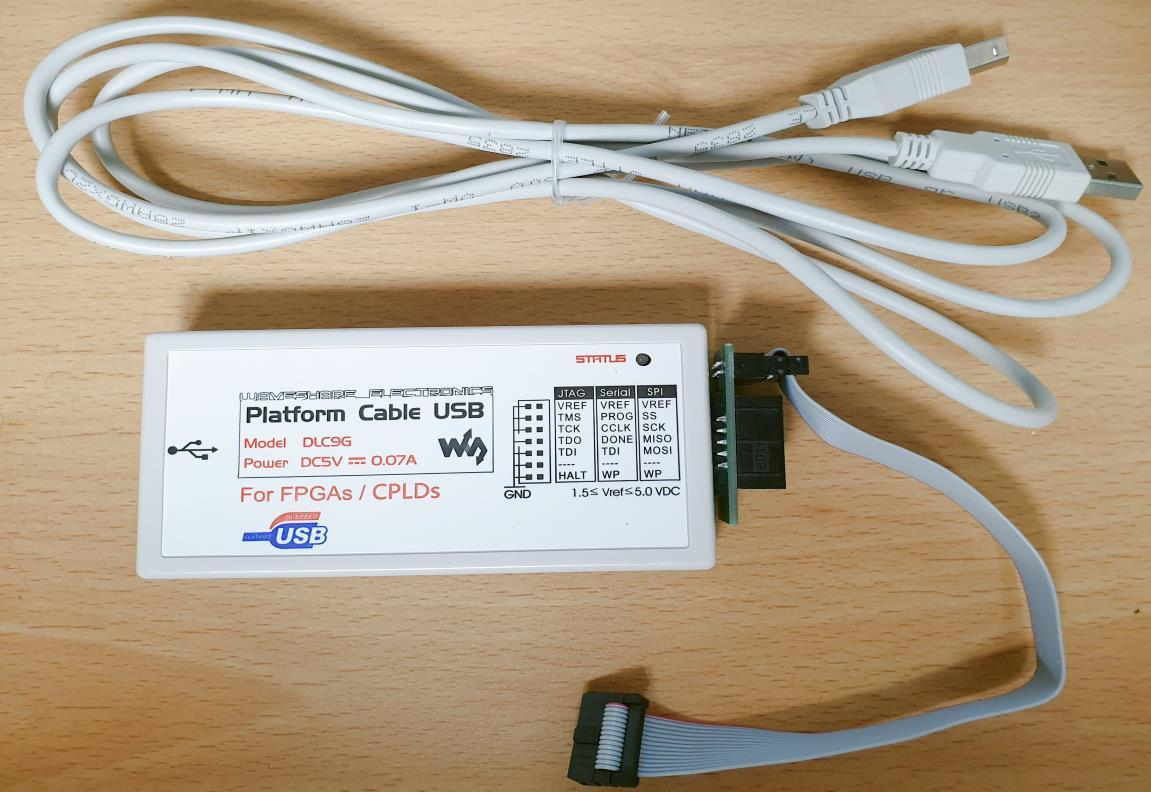
\includegraphics[width=\textwidth,height=4.6cm,keepaspectratio]{assets/legacy-01/p046-01.jpg}
\par}
\legacySource{46}
\end{frame}

\begin{frame}[label=legacy-01-p47]{로직 설계 및 합성}
\small
{\color{UOSBlue}\bfseries (6) Programming}\par\vspace{0.12cm}
\begin{itemize}
\setlength{\itemsep}{0.08cm}
\item {장비의 전원이 꺼져 있는지 확인}
\item {Xilinx Platform Cable에 USB Cable의 한 쪽 끝을 연결}
\item {반대쪽 끝은 PC의 USB 포트에 연결}
\item {Xilinx Platform Cable에 연결된 2x14핀의 플랫 케이블은 장비의 Xilinx 모듈의 JTAG 포트에 연결}
\item {장비의 전원을 켠다.}
\end{itemize}
\legacySource{47}
\end{frame}

\begin{frame}[label=legacy-01-p48]{로직 설계 및 합성}
\small
{\color{UOSBlue}\bfseries (6) Programming}\par\vspace{0.12cm}
\begin{itemize}
\setlength{\itemsep}{0.08cm}
\item {Xilinx Platform II Cable을 PC에 연결한 후, PC의 장치관리자에서 장치 인식 확인}
\end{itemize}
\par\vspace{0.12cm}
{\centering
\includegraphics[width=\textwidth,height=4.6cm,keepaspectratio]{assets/legacy-01/p048-01.png}
\par}
\legacySource{48}
\end{frame}

\begin{frame}[label=legacy-01-p49]{로직 설계 및 합성}
\small
{\color{UOSBlue}\bfseries (6) Programming}\par\vspace{0.12cm}
\begin{itemize}
\setlength{\itemsep}{0.08cm}
\item {Open Target \textgreater{} Auto Connect}
\end{itemize}
\par\vspace{0.12cm}
{\centering
\includegraphics[width=\textwidth,height=4.6cm,keepaspectratio]{assets/legacy-01/p049-01.png}
\par}
\legacySource{49}
\end{frame}

\begin{frame}[label=legacy-01-p50]{로직 설계 및 합성}
\small
{\color{UOSBlue}\bfseries (6) Programming}\par\vspace{0.12cm}
\begin{itemize}
\setlength{\itemsep}{0.08cm}
\item {Program Device 선택}
\end{itemize}
\par\vspace{0.12cm}
{\centering
\includegraphics[width=\textwidth,height=4.6cm,keepaspectratio]{assets/legacy-01/p050-01.png}
\par}
\legacySource{50}
\end{frame}

\begin{frame}[label=legacy-01-p51]{로직 설계 및 합성}
\small
{\color{UOSBlue}\bfseries (6) Programming}\par\vspace{0.12cm}
\begin{itemize}
\setlength{\itemsep}{0.08cm}
\item {Bitstream File 선택}
\item {\textless{}Project Folder\textgreater{} \textbackslash{} logic\_gate.runs \textbackslash{} impl\_1 \textbackslash{} logic\_gate.bit 파일 선택}
\item {Program 버튼 클릭}
\end{itemize}
\legacySource{51}
\end{frame}

\begin{frame}{로직 설계 및 합성}
\small
{\color{UOSBlue}\bfseries (6) Programming}\par\vspace{0.12cm}
{\scriptsize 원문 설명에 대응하는 실제 화면}\par
\par\vspace{0.12cm}
{\centering
\includegraphics[width=\textwidth,height=4.6cm,keepaspectratio]{assets/legacy-01/p051-01.png}
\par}
\legacySource{51}
\end{frame}

\begin{frame}[label=legacy-01-p52]{로직 설계 및 합성}
\small
{\color{UOSBlue}\bfseries (7) 동작 확인}\par\vspace{0.12cm}
\begin{itemize}
\setlength{\itemsep}{0.08cm}
\item {SW 1와 SW 2를 눌러 장비에서 어떻게 동작하는지 확인.}
\end{itemize}
\legacySource{52}
\end{frame}

\begin{frame}[label=legacy-01-notes]{보충 · 원문 표기와 실행 조건}
\small

\begin{itemize}
\setlength{\itemsep}{0.3cm}
\item 원본 p.24--25의 \texttt{LVCMOSS33}은 오타다.\par
실제 I/O 표준은 \texttt{LVCMOS33}을 선택한다.
\item \texttt{d:/work}는 원본의 예시 작업 경로다.\par
실제 프로젝트를 저장한 경로를 사용한다.
\item 원본 테스트벤치는 10 ns 단위에서 \texttt{\#20}마다\par
입력을 바꾼다. 입력 전환 간격은 200 ns다.
\item 원본의 \texttt{a,b} 입력 순서는 00, 10, 01, 11이다.\par
출력 \texttt{x,y,z}를 AND·OR·XOR 진리표와 비교한다.
\end{itemize}
\vspace{0.3cm}
{\scriptsize 이 페이지는 원본과 구분한 보충 설명이다. 원본 코드 이미지는 유지했다.}

\end{frame}

\begin{frame}[label=legacy-01-prelab]{보충 · VS Code 사전 시뮬레이션}
\small

\begin{enumerate}
\setlength{\itemsep}{0.23cm}
\item \texttt{logic\_gate.v}와 테스트벤치를 VS Code에서 연다.
\item 배포 workspace의 02 Simulate로 자기검사 TB를 실행한다.
\item 원본 테스트벤치에는 자동 종료·VCD 저장 구문이 없다.\par
사전 실습은 별도 TB로 4개 입력·40 ns와 VCD를 검사한다.
\item 생성한 파형에서 \texttt{a,b,x,y,z}를 확인하고 예상값과 비교한다.
\item 실행 방법·코드 설명·파형 해석을 실험 전 레포트에 쓴다.
\end{enumerate}
\vspace{0.3cm}
{\scriptsize \href{02.vscode_verilog_환경설정_매뉴얼.pdf}{VS Code 환경설정 매뉴얼} ·
\navlink{lab1-reports}{레포트 안내}\par
사전 단계는 이번 수업의 보충 안내이며 원본 Vivado 화면과 구분한다.}

\end{frame}

\begin{frame}[label=legacy-01-postlab]{보충 · 보드 결과와 실험 후 레포트}
\small

\begin{enumerate}
\setlength{\itemsep}{0.22cm}
\item Vivado 파형을 VS Code 사전 시뮬레이션과 비교한다.
\item 생성한 \texttt{logic\_gate.bit}를 실제 FPGA에 기록한다.
\item SW\_1·SW\_2의 네 입력 조합과 LED1·LED2·LED3를 확인한다.
\item 연결 상태는 사진, 입력에 따른 출력 변화는 영상으로 남긴다.
\item 코드·파형·사진·영상을 GitHub에 올리고 레포트에 연결한다.
\end{enumerate}
\vspace{0.35cm}
실제 결과와 예상값을 비교하고 오류·수정 사항을 설명한다.\par
\vspace{0.2cm}
{\scriptsize 원본 화면의 성공 표시와 본인의 실행 결과를 구분한다.\par
\navlink{legacy-01-contents}{이 실습 목차} · \href{04.LAB1_00_CONTENTS.pdf}{전체 목차 PDF}}

\end{frame}
